\section{Compute resources: access and provisioning}
\label{computeresources}


End-user data analysis workflows are evolving significantly, with new data formats designed by the LHC collaborations to reduce the storage footprint and be more compatible with modern data science paradigms, eventually enabling researchers to utilize frameworks that require little to no experiment-specific software. This evolution will have an impact on the infrastructure and resources dedicated to user analysis activity.

Outlined are the current R\&D activities that have been reported to the HSF AF forum, with particular focus on the evolution of access and provisioning of the compute resources to expose heterogeneous and possibly distributed resources. A set of recurrent questions and discussions are the starting point for the review targeted by this section: 
\begin{enumerate}
    \item \textbf{Compute resources access:}
    \begin{enumerate}[label=(\alph*)]
        \item Workflow management: tools leveraging batch systems in a native way are arguably the most widely adopted ones at the time of writing, nevertheless workflows are becoming larger and more complicated and the integration of cloud paradigms for a seamless transition from local “interactive” development to full scale analysis multi-step execution are emerging in many R\&D activities. That is expected to enable enhanced data exploration and reduce “time-to-insight”.
        \item UX/UI: ssh-ing into a preconfigured machine is a de-facto standard for most analysis and that is not expected to change. Instead, a possible enhancement of the UX is expected to come from WebUI interfaces largely adopted in the context of cloud/notebook based data science ecosystems.
        \item 
        AAI: the adoption of tokens for Authentication and Authorization by the HEP community is also important in the context of AFs and integration of cloud technologies as well as simplified access to data from diverse resources. Section~\ref{aai} is dedicated to AAI infrastructure.
        \item Containers: a base hypothesis of the computing models under investigation is that the payloads are containerized. Section~\ref{preservation} details the portability and reproducibility of that approach.
    \end{enumerate}
    \item \textbf{Compute resources provisioning:}
    \begin{enumerate}[label=(\alph*)]
        \item Provisioning responsiveness: point 1.a shows a significant shift in terms of the latency that is acceptable in the interactive vs. non-interactive scenarios. That opens the question of how to implement a computing model at AF level where dynamic provisioning can possibly live alongside crowded traditional batch systems.
        \item Efficiency and performance: upcoming frameworks that are enabling a whole set of new possibilities from the user perspective have to be validated against their efficiency in terms of resource utilization and overall physics throughput. 
        \item Site provisioning model: HPC centers and commercial clouds are going to have a significant impact on the future of resource provisioning. Finding a way to integrate them seamlessly is crucial, along with the understanding of which kind of analysis paradigm can benefit the most from that integration. 
        \item Resource provisioning model: the server level is the other side of the spectrum of the provisioning model. One solution could be to allocate whole nodes and reserve a whole “fat” node that is fully committed to achieve the quickest analysis turnaround time. It remains to be seen if this can be sustainable in the future and compatible with the goal of maximum overall resource efficiency.
        \item Specialized hardware: the adoption of GPUs and, potentially, FPGA acceleration, is expected to increase, and this has to be made both easy and efficient from the infrastructure perspective. Although not many case studies have been reported, we do expect this to be a strategic point to investigate. This is transversal to both access and provisioning patterns. 
    \end{enumerate}
\end{enumerate}





 


Many R\&Ds reported to the AF Forum on their investigations, which allows an “educated guess” on what the main traits are for future analysis infrastructures. 

\subsection*{User Interfaces}

The SSH login into a pre-configured UI still holds as a requirement for many use cases, especially for non-pythonic workflows like scripting for batch job submission. For analysis of reduced data (at the moment often done in the previous step), an interactive interface can be accessed through the adoption of tools enabling a single WebUI to log in and access the resources they need. JupyterHub is a popular choice for this, because it allows multiple users to spawn JupyterLab instances on a cluster of servers. One interesting model emerged for point 2.a: providing users with a relatively small amount of “always-on” resources, ready to get the user started with an interactive workflow, while scheduling a larger fraction on lazier batch system queues, leveraging offloading mechanisms (see below). Another area of investigation is the possibility of using JupyterHub as a mechanism for ssh-UI on-demand provisioning, integrating the SSH access into a running JupyterLab instance, thus enabling users to share a common environment with access to different UIs.

\subsection*{Offloading to external resources}
In terms of supporting the offloading of “heavy lifting” workflows to external resources, and since the possibility to distribute batch jobs is still a requirement, most of the reported activities aim to integrate a mechanism for leveraging the batch systems as an offloading backend for the more “interactive”/data-science-like analysis workflows. That behavior has been demonstrated mostly via Dask cluster deployments. In fact, many of the presented solutions have their foundation in Dask distributing payloads on either HTCondor~\cite{htcondor} or SLURM~\cite{slurm}. Some sites have deployed Apache Spark~\cite{spark} managed clusters, notably CERN Analytix cluster. For the requirements of fast prototyping of ML models and even full analyses, an offloading mechanism for a whole JupyterLab instance to a remote, specialized node that is fully committed to the analysis for a short period of time could be considered. Although possible, it has yet to be proven sustainable at scale with dedicated activities. With all of these considerations in mind,  figure~\ref{fig:AFschema} attempts to schematize a high level description of an AF resource management “strawman”. 

Different models for the evolution of the access and provisioning of analysis resources have been presented by several groups (SWAN~\cite{swan}, Coffea Casa~\cite{coffea}, NAF~\cite{NAF}). Most of the commonalities are in the methods of providing access to the users’ UIs. Providing SSH and/or JupyterHub access is becoming a default mode of operations in many (if not all) the presented activities. Interesting variations occur for the scale-out mechanism toward remote resources. A number of facilities have the batch resources co-located (in terms of network segregation) with the AF interactive seed, differing only in the integration with the analysis tools. On a slightly different path, there is an evaluation for integrating geo-distributed centers (e.g.,T2 grid resources) as offload candidates for tasks (INFN~\cite{INFN_distributed}); this presents the problem of having the JupyterLab instance on a different network from the worker nodes. The current solution in such a scenario is the creation of a self-contained cluster to be created at the remote site on-demand. 

\begin{figure}
    \centering
    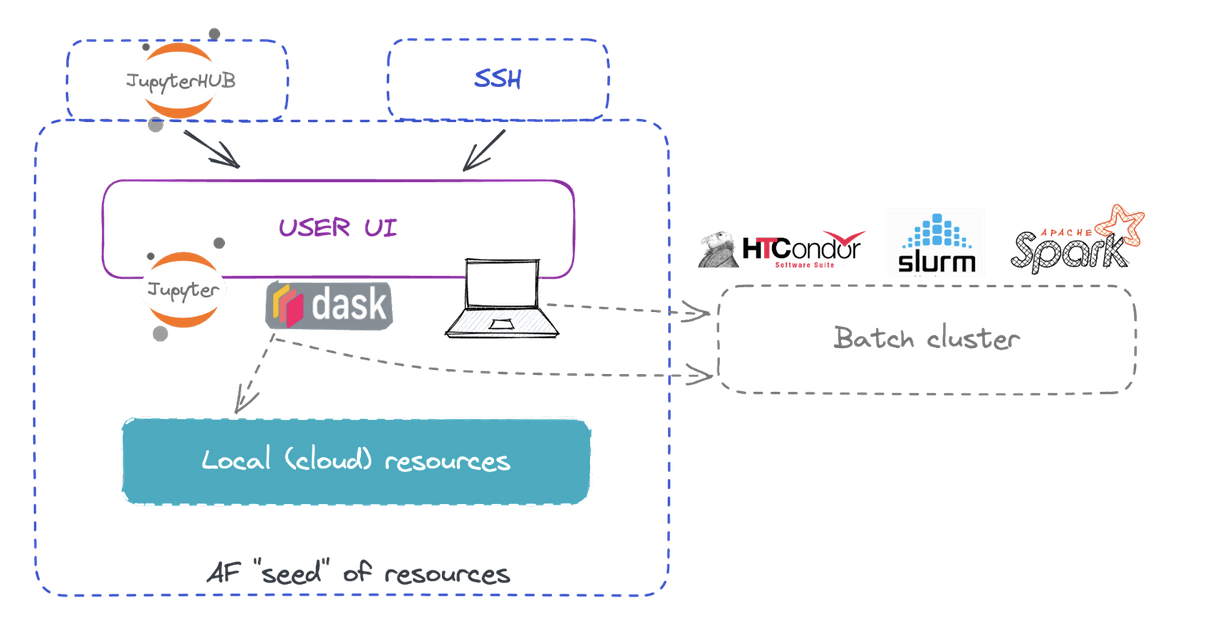
\includegraphics[height=6cm]{fig/schema.png}
    \caption{High level schema of the recurrent patterns reported at the forum by R\&D activities around compute access and provisioning models evolution.}
    \label{fig:AFschema}
\end{figure}

One final observation is that there are ongoing efforts, presented by the kubernetes~\cite{k8s} user activities, that might allow for an alternative implementation. Here, payloads and their distribution can eventually be fully delegated to kubernetes native resources with the introduction of dedicated abstractions and scaling improvements. There are preliminary implementations and R\&D efforts that have been reported at the forum but have yet to be investigated properly in order to make a clear comparison with the alternatives presented above.

To support complicated workflow pipelines, as expressed in the user requirements, workflow languages such as Snakemake~\cite{snakemake}, Yadage~\cite{yadage}, Common Workflow Language (CWL)~\cite{cwl} and others may be suitable. Also, some workload schedulers have features that allow users to express dependencies between workloads (e.g. HTCondor's tool DAGMan). Workflow services such as REANA~\cite{reana}, capable of processing such languages, should be integrated into the existing batch infrastructure at the facility in order to have access to the same data and compute resources that would be available if the pipeline were processed manually. Note that REANA also works with a kubernetes back end. 

\subsection*{Open Questions}

\subsubsection*{On resource interoperability?} If we cannot guarantee uniformity of technologies how do we manage “interoperability” between resource providers?

\subsubsection*{On a common interface}

Given the large number of new technologies should users be exposed to all of these or should there be a common entry point interface such as JupyterLab? Reaching agreement on a common interface will be challenging, the introduction of Jupyter Notebooks/JupyterLab is an attempt at having a common interface but this remains an open question. 


